% SPDX-License-Identifier: Apache-2.0
\section{Lerneinheiten: vom Lernversprechen zum rekursiven Abschluss}
\label{sec:learning-units}
\begin{principle}{Fachliche Einheit statt Kalenderschublade}
Eine \textbf{Lerneinheit} (englisch \emph{learning unit}, künftiger
technischer Begriff \code{LearningUnit}) verbindet ein verständliches
Lernversprechen mit eigenen Lernzielen und gegebenenfalls kleineren
Lerneinheiten. Die Struktur ist rekursiv: Mechanik kann Kinematik und
Dynamik enthalten; Kinematik kann ihrerseits weitere Einheiten enthalten.
Schuljahr, Semester und Lernwoche sind mögliche Planungsbezüge, keine
Synonyme für eine Lerneinheit. Personalisierungslevel 1--4, QA-Reifegrade
und das Schwierigkeitsfeld \code{level} behalten ihre bisherige Bedeutung.
\end{principle}

\subsection{Motivation und eigener fachlicher Anspruch}
Die Einheit beantwortet zuerst: \emph{Was kann ich danach, und wozu ist
das nützlich?} Ein Motivationsauftakt macht dieses Versprechen verständlich,
bevor einzelne Aufgaben oder Ziele angeboten werden. Der Auftakt ist eine
didaktische Funktion. Wenn er als echtes Orientierungsziel modelliert ist,
gilt dessen eigener Ergebnisvertrag; eine synthetische Überschrift ist
dadurch kein zusätzliches Lernziel. Aus einem abgeleiteten Abschluss folgt
keine Behauptung, dass ein Motivationsgespräch tatsächlich stattgefunden hat.

Eine größere Einheit kann vorhandene Kindkompetenzen nur zusammenfassen.
Dann braucht sie keine neue eigene Prüfung. Verspricht sie zusätzlich deren
selbstständige Integration, kann eine eigene Syntheseprüfung diesen Anspruch
prüfen. Sie kann sich dabei auf bereits in Kindern erworbene Kompetenzen
beschränken. Zusätzliche eigene Fachkompetenzen sind ebenfalls möglich;
sie brauchen ihre eigene Erwerbszuordnung und gültige Prüfungsdeckung.
Für reine Synthese müssen keine künstlichen neuen gewöhnlichen Ziele
erfunden werden. Ihre Rolle ist der zusätzliche Integrationsnachweis, nicht
das erneute Bestehen aller Kinder.

\subsection{Direkter Erwerb, Kinder und Gesamtumfang}
Für eine autoritative, versionierte Einheit U bezeichnet $\Own(U)$ die
direkt zugeordneten atomaren Erwerbsziele. Echte Orientierungs-, Prüfungs-
und Memorierziele können dazugehören; reine Strukturmarker nicht.
$\Children(U)$ enthält die verpflichtenden Kindlerneinheiten. Wahlentscheidungen
sind zuvor aufgelöst. Die eindeutige gesamte Zielmenge ist
\begin{equation}
 T(U)=\Own(U)\cup\bigcup_{V\in\Children(U)}T(V).
 \label{eq:unit-targets}
\end{equation}
Der aufgelöste Gesamtumfang ist nicht leer. Ein leerer Navigationsmarker
ist keine abgeschlossene Lerneinheit. Ein Aggregat darf dagegen leere
eigene Ziele haben, wenn seine Pflichtkinder den Gesamtumfang tragen.
Jeder Ersterwerb ist auf der kleinsten fachlich zuständigen autoritativen
Einheit verortet. Eine Elternansicht darf dieselben stabilen Ziele zeigen,
ohne sie erneut als eigene Erwerbsziele zu beanspruchen. Überlappende
Referenzen werden als Mengen vereint; sie erzeugen weder zusätzliche Ziele
noch doppelte Fortschrittspunkte. Ein bloßer Fokuswechsel verändert diese
Zuordnung und ihren Anerkennungsvertrag nicht.
Jedes gewöhnliche fachliche Ziel in $\Own(U)$ braucht einen eigenen lokalen
Prüfungsverbraucher und unabhängig geprüfte Anwendungsdeckung in Aufgabe
und normaler Rubrik. Ohne diese Deckung ist der Erwerbsvertrag ungültig;
eine zusätzliche frei gewählte Anerkennungsmaske ist kein Ersatz.

Die Einbettung benutzt die vorhandene Program-/Placement- beziehungsweise
geprüfte Composition-Struktur. Eine fachliche Einheit ist nicht allein
deshalb definiert, weil ein Cluster gerade aufgeklappt ist. Ebenso wenig
wird jeder beliebige \code{contains}-Cluster automatisch zur Lerneinheit.
Insbesondere bleibt die allgemeine Clustererfüllung aus dem Kernkapitel
von der hier erklärten, ausdrücklich autorisierten Einheitsstruktur
unterschieden.

\subsection{Abschluss ohne zusätzlich gespeicherte Unit-Mastery}
Die vollständige Einheit ist abgeschlossen genau dann, wenn ihre eigenen
Ziele erfüllt und alle verpflichtenden Kinder abgeschlossen sind:
\begin{equation}
 \Complete(U)\iff
 \bigl(\Own(U)\subseteq M_{\mathrm{eff}}\bigr)\ \land\
 \bigwedge_{V\in\Children(U)}\Complete(V).
 \label{eq:unit-complete}
\end{equation}
Prüfungs- und Memorierziele bleiben ausschließlich explizit. Daher kann
eine bestandene Elternprüfung keine offene Kindprüfung und keinen fehlenden
verifizierten Kartenabruf ersetzen. Es entsteht keine gespeicherte
\code{UnitMastery}, die Ergebnisse auf Kinder zurückschreibt.

Ein reines Aggregat darf ohne eigene Prüfung bestehen: Sein Abschluss folgt
aus den Kindern und eventuell anderen eigenen Pflichten. Eine Syntheseeinheit
kann dagegen eine eigene Prüfung, aber keine neuen gewöhnlichen Erwerbsziele
haben. Ihre Prüfung ist dann zusätzlich erforderlich. Eine reine Kartensammlung
begründet keinen Anspruch unabhängiger fachlicher Anwendung; ihre tatsächlichen
Abrufpflichten bleiben ausdrücklich zu erfüllen. Eine fachlich zum Kind
gehörige Recallpflicht darf nicht allein zur Erzeugung eines Kindabschlusses
auf die Eltern verschoben werden.

\begin{figure}[htbp]\centering
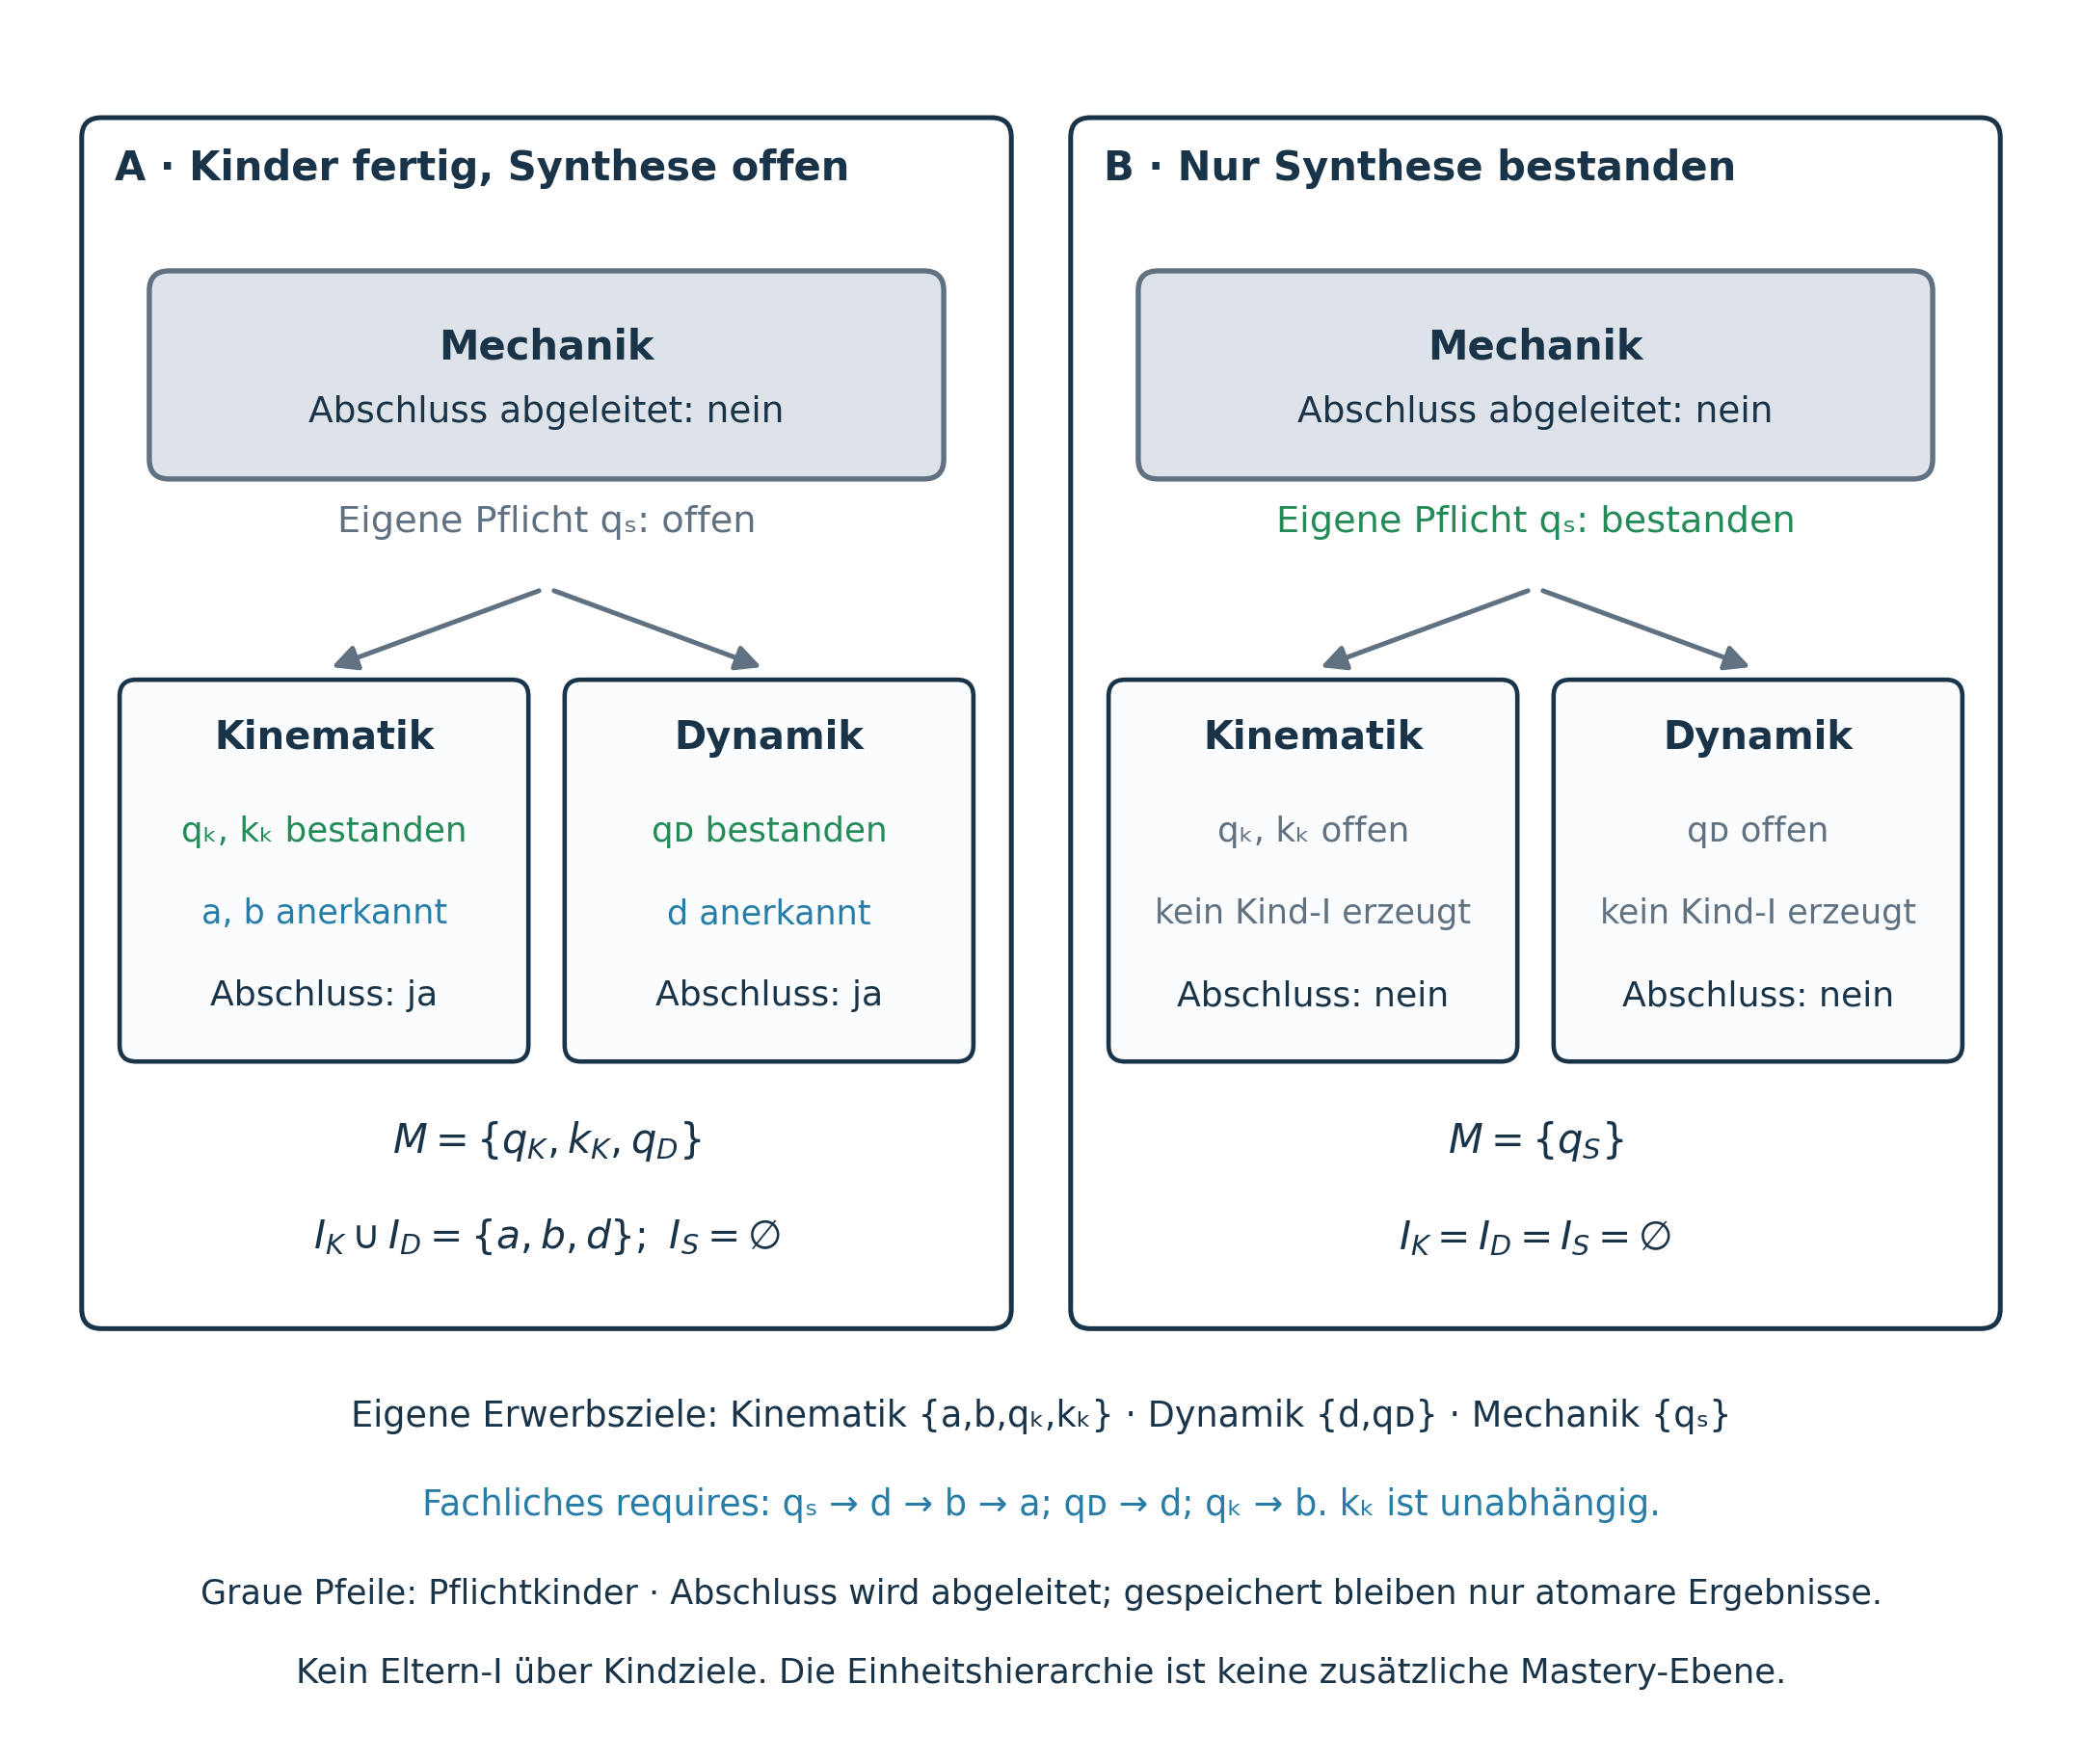
\includegraphics[width=\linewidth]{assets/graph-definition/16-recursive-learning-unit.png}
\caption[Mechanik als rekursive Lerneinheit]{Illustrative Hierarchie mit
eigenständigen Kindverträgen. Links sind beide Kinder vollständig
abgeschlossen, ihre Kompetenzen global anerkannt; die offene Synthese
hält allein den Elternabschluss offen. Rechts ist nur die Elternprüfung
bestanden. Sie erzeugt keine Kindprüfungen, keinen Kartenabruf und keine
Anerkennung der Kindkompetenzen. Graue Pfeile zeigen ausschließlich die
Einheitshierarchie; die fachlichen Kanten stehen getrennt darunter.}
\label{fig:recursive-unit}\end{figure}
\FloatBarrier

\subsection{Anerkennung vor dem Gesamtabschluss}
Eine passende bestandene Prüfung kann die eigenen gewöhnlichen Kompetenzen
einer Einheit anerkennen, bevor eine davon unabhängige Karte oder ein anderes
Kind abgeschlossen ist. Diese Anerkennung ist global wirksam. Eine noch
offene Syntheseprüfung der Eltern nimmt sie nicht zurück.

Für jede Einheit wird deshalb nur die Anerkennung ihrer \emph{eigenen}
gewöhnlichen Erwerbsziele berechnet. Die Eltern bilden aus allen Nachfahren
keinen neuen vergrößerten Anerkennungsumfang. Sonst könnte ihre Prüfung
untergeordnete Prüfungs- oder Kartenpflichten unzulässig umgehen.
Eine Elternprüfung kann zusätzliche Integration belegen, ohne die
ursprüngliche Nachweisbedeutung der Kindverträge rückwirkend zu erweitern.
Die genaue Bedarfsformel und ihre Inhaltsbedingungen stehen in
Abschnitt~\ref{sec:assessment}.

\subsection{Voraussetzungen und die Grenze einer Einheitsfolge}
Eine ausdrücklich autorisierte Voraussetzung zwischen ganzen Lerneinheiten
bedeutet \emph{Vollabschluss} der vorausgesetzten Einheit. Ein atomarer
\code{requires}-Bezug auf eine Kompetenz fordert dagegen diese Kompetenz;
er fordert nicht automatisch den Abschluss ihrer gesamten Einheit.
Die Ganzheitsvoraussetzung gehört zum Kompositionsvertrag außerhalb der
bisherigen Grundrelationen C und R. Diese Aussagen dürfen weder im Compiler
noch im Coach verwechselt werden.

Die Einheitshierarchie muss azyklisch sein. Wer darüber hinaus eine
ungeteilte Abschlussfolge von Einheiten behauptet, muss auch deren
Voraussetzungsgraphen prüfen. Ein atomarer DAG genügt nicht: Bei
$a\to b\to c$, $\Own(U)=\{a,c\}$ und $\Own(V)=\{b\}$ entsteht nach
Zusammenfassung eine Abhängigkeit in beide Richtungen. U und V sind so
keine gültige ungeteilte Vollabschlussfolge. Die Diagnose erfordert eine
andere Gruppierung oder einen ausdrücklich feineren Erwerbsablauf;
sie erzeugt keine stillschweigenden Ganzheitssperren aus atomaren Kanten.
Die bestehende transitive Minimalität gilt weiterhin für verfasste
\code{requires}-Kanten unter neu berechneter effektiver Vererbung und
atomarer Expansion. Daraus folgt noch keine neue Minimalitätsregel für
eine erst zu beschließende Ganzheitszugangsrelation.

\begin{principle}{Zugangsprofil noch offen}
Eine fachliche Erwerbsordnung ist noch keine technische Zugangssperre.
Ob und wann ein ausdrücklicher Einheitsbezug einen harten Zugangsschutz
erzwingt, und wie dann direkte Prüfungsversuche behandelt werden, ist
\textbf{noch nicht entschieden}. Ein solches Profil wäre gesondert zu
beschließen und zu prüfen. Die Einheitendefinition führt es nicht ein.
\end{principle}

Nur \emph{falls} später ein ausdrückliches Sperrprofil gewählt wird, könnte
man für autorisierte Vorgängereinheiten $\operatorname{Pred}(U)$ definieren:
\[
 \operatorname{Open}(U)=\bigwedge_{V\in\operatorname{Pred}(U)}
      \operatorname{Cleared}(V),\qquad
 \operatorname{Cleared}(U)=\operatorname{Open}(U)\land\Complete(U).
\]
$\Complete$ beschreibt die vorhandenen Nachweise, $\operatorname{Cleared}$
nur die bedingte Kurspolitik. Weder das Öffnen noch diese abgeleitete
Freigabe vergibt Mastery. Ob direkte Prüfungen bei geschlossenem Zugang
zulässig bleiben, entscheidet diese bloße Beispielgleichung nicht.

\paragraph{Quellen.}
\srcref{docs/concept/skill-graph/learning-units.md}{Lerneinheiten};
\srcref{docs/concept/skill-graph/learning-unit-progression.md}{Einheitsfolge und Zugangsprofile};
\srcref{docs/concept/skill-graph/graph-definition.md}{Graph Definition, Abschnitt 12};
\srcref{docs/concept/skill-graph/assessment-gated-completion.md}{Anerkennung und globaler Abschluss}.
